Now we can start to see some interesting examples for a complete understanding of our technique and of software functionalities. In the example that we will introduce in this chapter, we will study in detail the output of every conversion step. In particular, here we will use one of the classic example of computer graphics: the \textbf{Stanford Bunny}. 
\begin{figure}[htb] %  figure placement: here, top, bottom
   \centering
   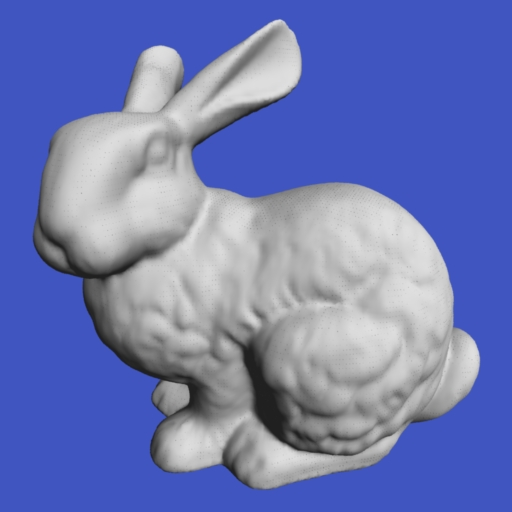
\includegraphics[width=0.30\linewidth]{images/stanfordBunny.jpg}
   \caption[A three-dimensional representation of the Stanford Bunny]{A three-dimensional representation of the Stanford Bunny (realized by Peter Lindstrom)}
   \label{fig:stanfordBunny}
\end{figure}

In the \textit{Stanford volume data archive} we can find a CT scan of a terra-cotta bunny which we will use to create our three-dimensional model. The data provided is in a raw $512\times512$ format with 361 slices stored as 16 bit pixels. First of all we have to read this data and create the images (the results are in Figure~\ref{fig:CTBunny}).

\begin{figure}[htb] %  figure placement: here, top, bottom
   \centering
   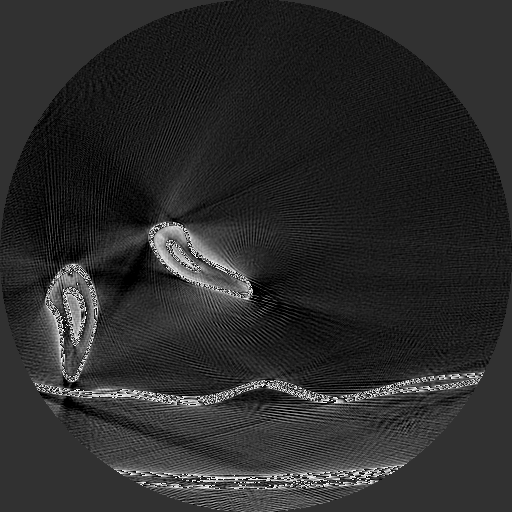
\includegraphics[width=0.30\linewidth]{images/CTBunny0.png}\hfill
   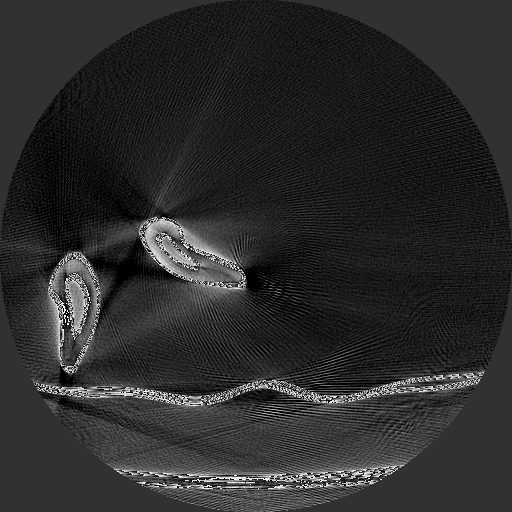
\includegraphics[width=0.30\linewidth]{images/CTBunny1.png}\hfill
   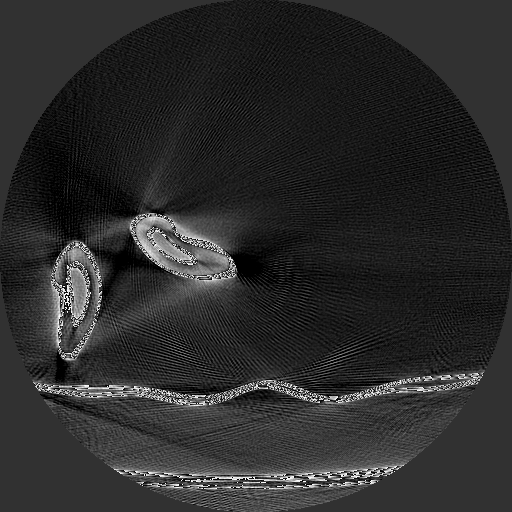
\includegraphics[width=0.30\linewidth]{images/CTBunny2.png}
   \caption[CT scans of the Stanford Bunny]{CT scans of the Stanford Bunny}
   \label{fig:CTBunny}
\end{figure}

At this point, we have to prepare the data for conversion. In particular, as we can see in Figure~\ref{fig:thrBunny}, we have applied a threshold on a data at the value of 37000 HU and a crop on y-axis cutting out the last 142 pixels and on z-axis cutting out 5 images:

\begin{figure}[htb] %  figure placement: here, top, bottom
   \centering
   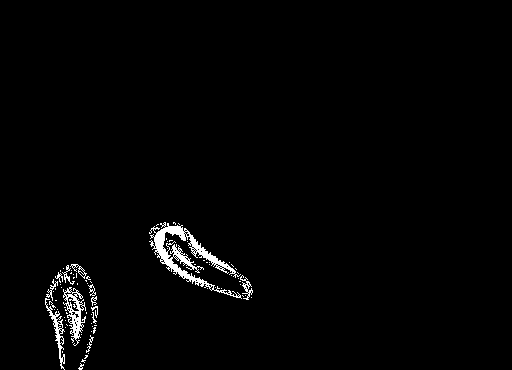
\includegraphics[width=0.30\linewidth]{images/thrBunny0.png}\hfill
   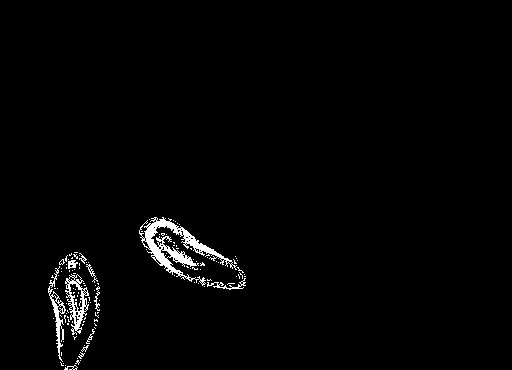
\includegraphics[width=0.30\linewidth]{images/thrBunny1.png}\hfill
   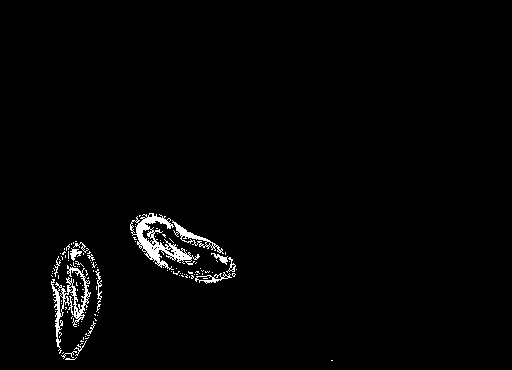
\includegraphics[width=0.30\linewidth]{images/thrBunny2.png}
   \caption[Binary images obtained from the previous CT scans]{Binary images obtained from the previous CT scans. Threshold set at 37000 HU}
   \label{fig:thrBunny}
\end{figure}

At the end of this step we have obtained 356 images with size $512\times370$, so now we can start the conversion pipeline. First of all we have to choose the sizes of the grid. In this case, we have chosen a grid of $64\times10\times4$. The first step consists in the computation of the boundary chain for every block. In Figure~\ref{fig:blockBunny} we can see two sample blocks

\begin{figure}[htb] %  figure placement: here, top, bottom
   \centering
   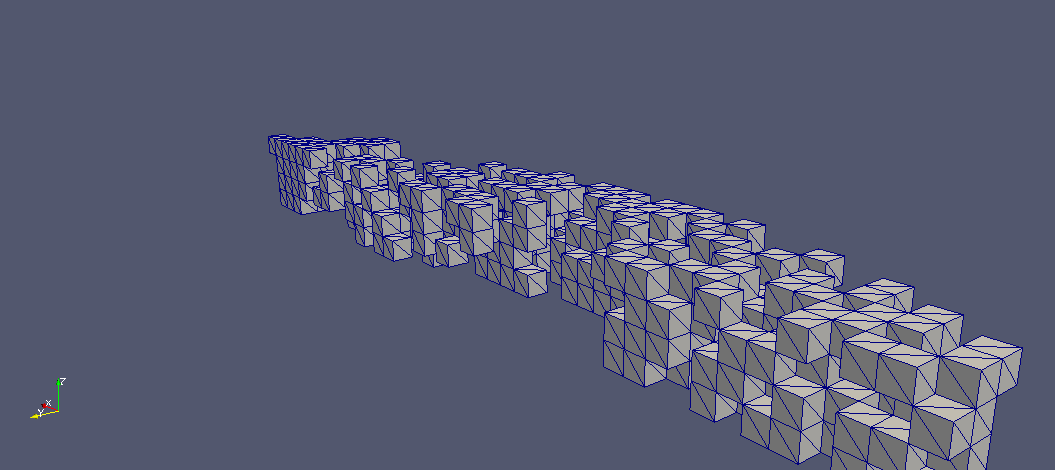
\includegraphics[width=0.49\linewidth]{images/Bunnyblock2.png}\hfill
   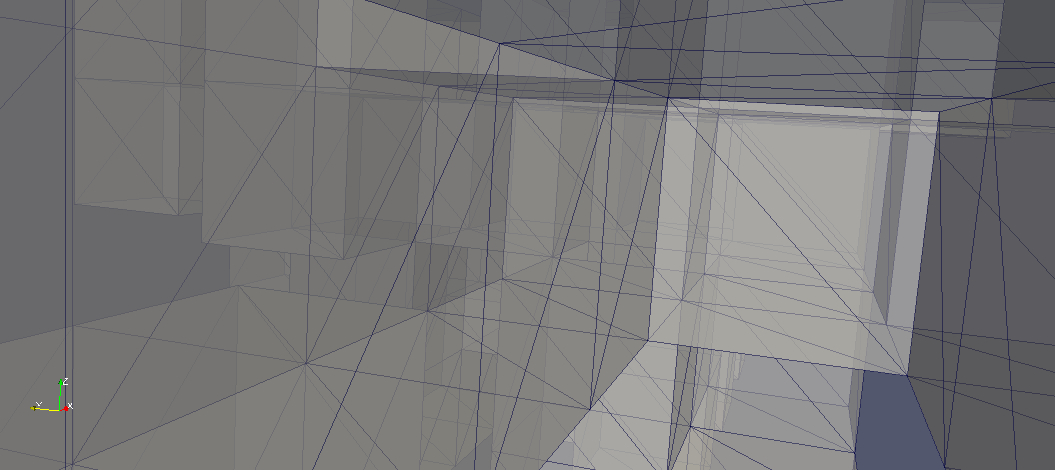
\includegraphics[width=0.49\linewidth]{images/Bunnyblock1.png}\newline
   
   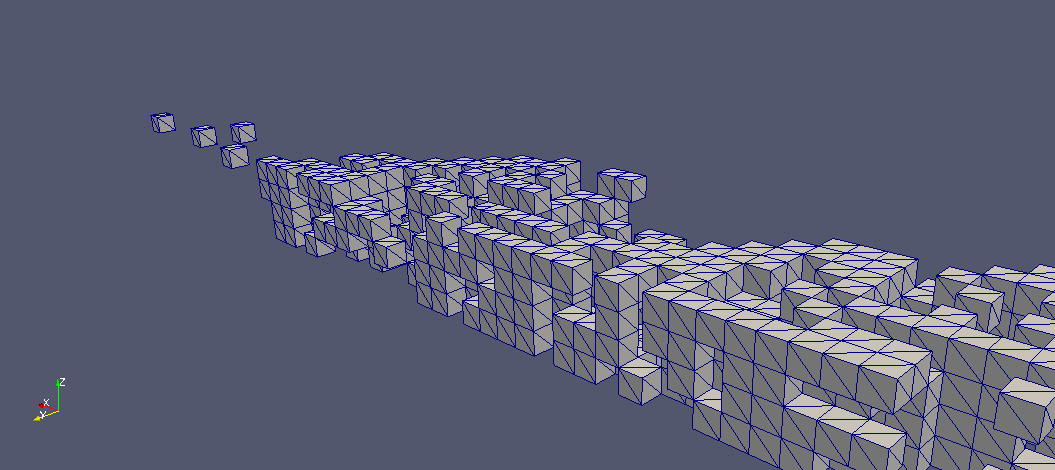
\includegraphics[width=0.49\linewidth]{images/Bunnyblock5.png}\hfill
   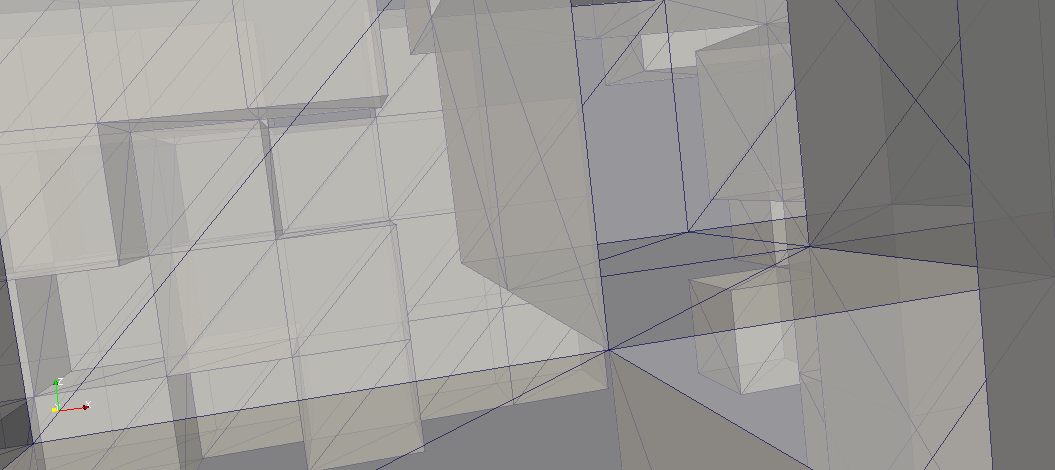
\includegraphics[width=0.49\linewidth]{images/Bunnyblock4.png}
   \caption[Some blocks obtained from the images]{Some blocks obtained from the images. On the two rows we have different sample blocks. Notice how every block is empty at its internal.}
   \label{fig:blockBunny}
\end{figure}

Now we can delete double vertices and boundaries between blocks. In Figure~\ref{fig:boundaryBunny} we can see the effect of the removal of the boundaries on the previous blocks.

\begin{figure}[htb] %  figure placement: here, top, bottom
   \centering
   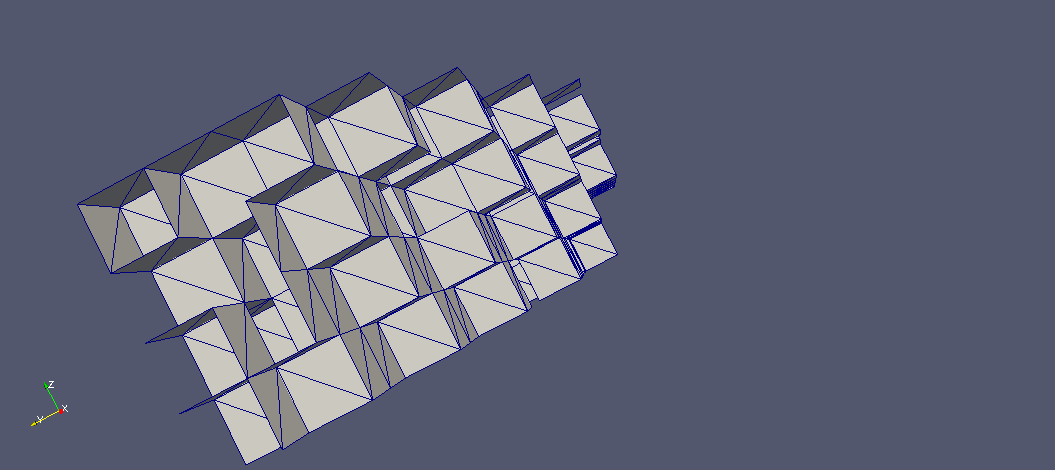
\includegraphics[width=0.49\linewidth]{images/BunnyNoBoundary0.png}\hfill
   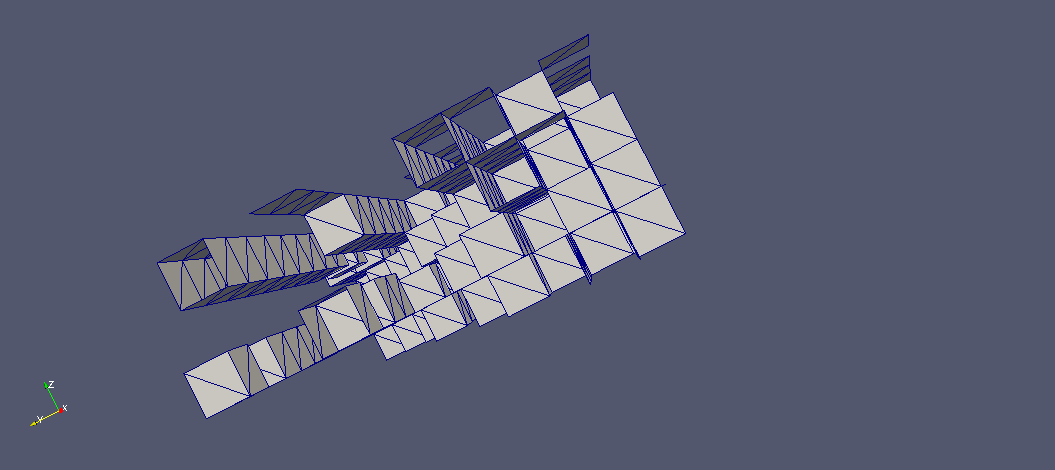
\includegraphics[width=0.49\linewidth]{images/BunnyNoBoundary1.png}
   \caption[Removal of duplicated boundaries from blocks]{Removal of the duplicated boundaries from blocks. The two figures refer to the two blocks in Figure~\ref{fig:blockBunny}}
   \label{fig:boundaryBunny}
\end{figure}

Now if we want to merge these blocks, we will obtain a three-dimensional model with squared edge (see Figure~\ref{fig:squaredBunny}).

\begin{figure}[htb] %  figure placement: here, top, bottom
   \centering
   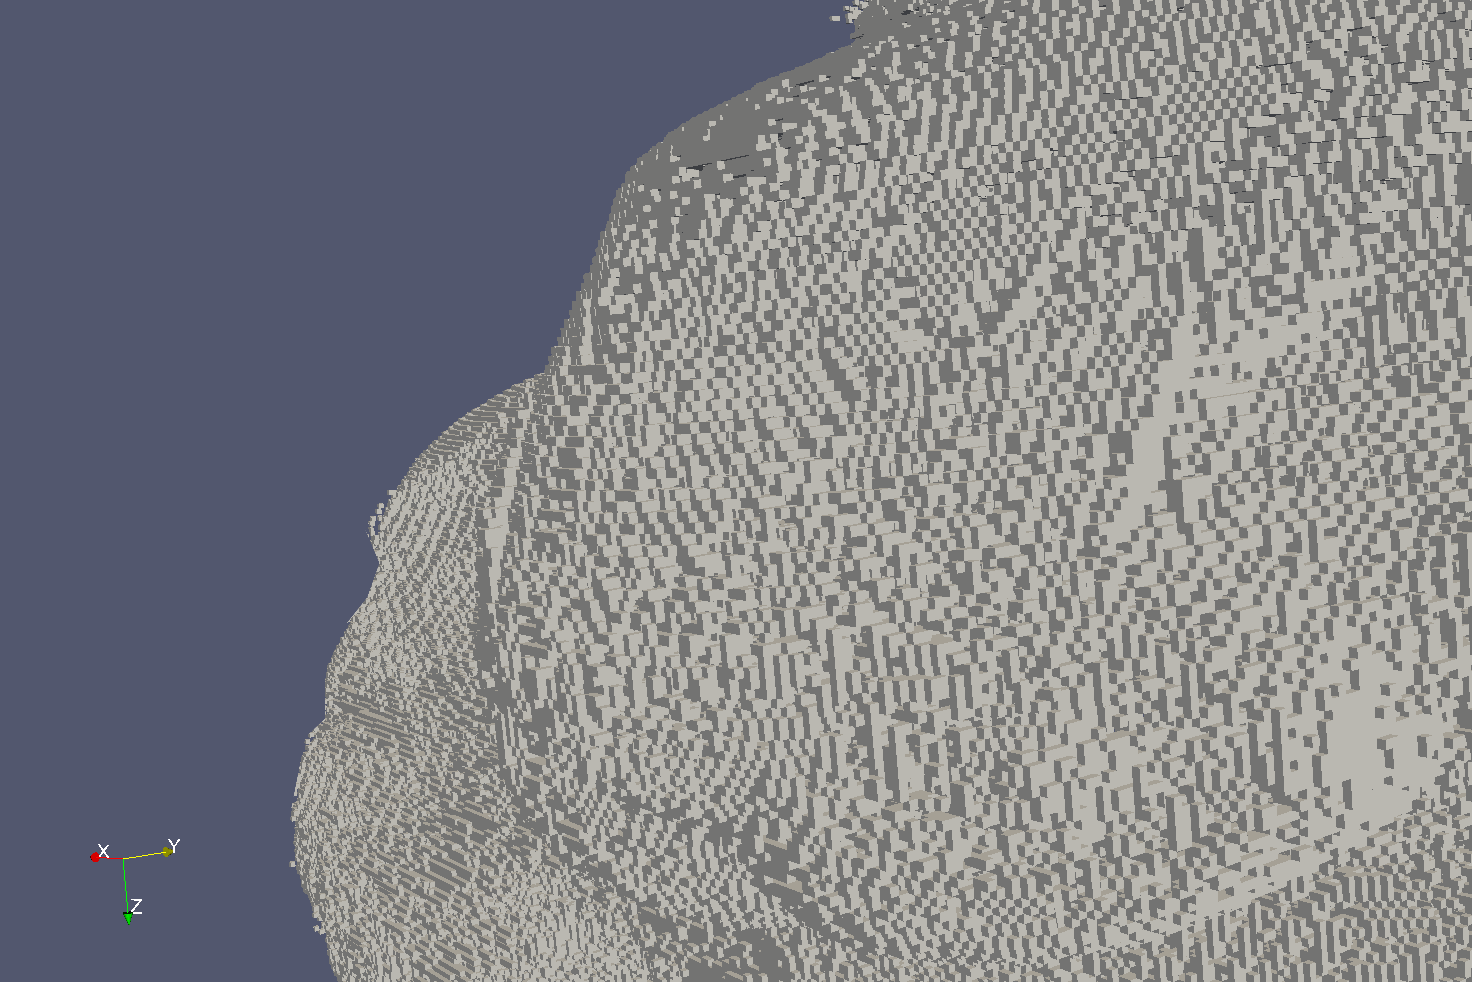
\includegraphics[width=0.49\linewidth]{images/nosmooth0.png}\hfill
   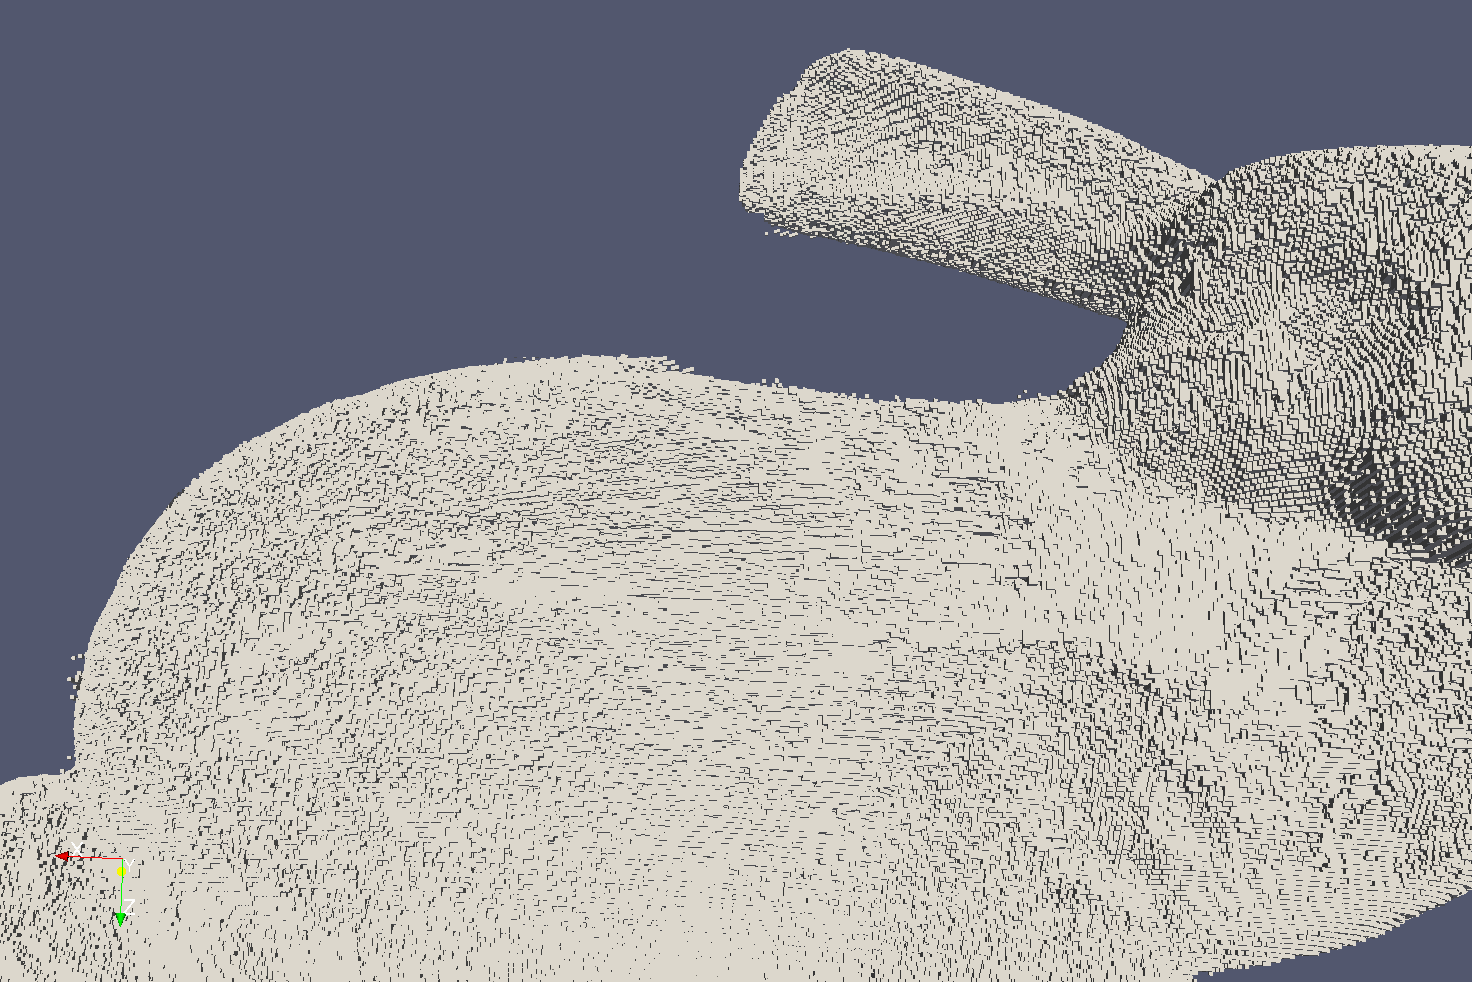
\includegraphics[width=0.49\linewidth]{images/nosmooth1.png}\newline
   
   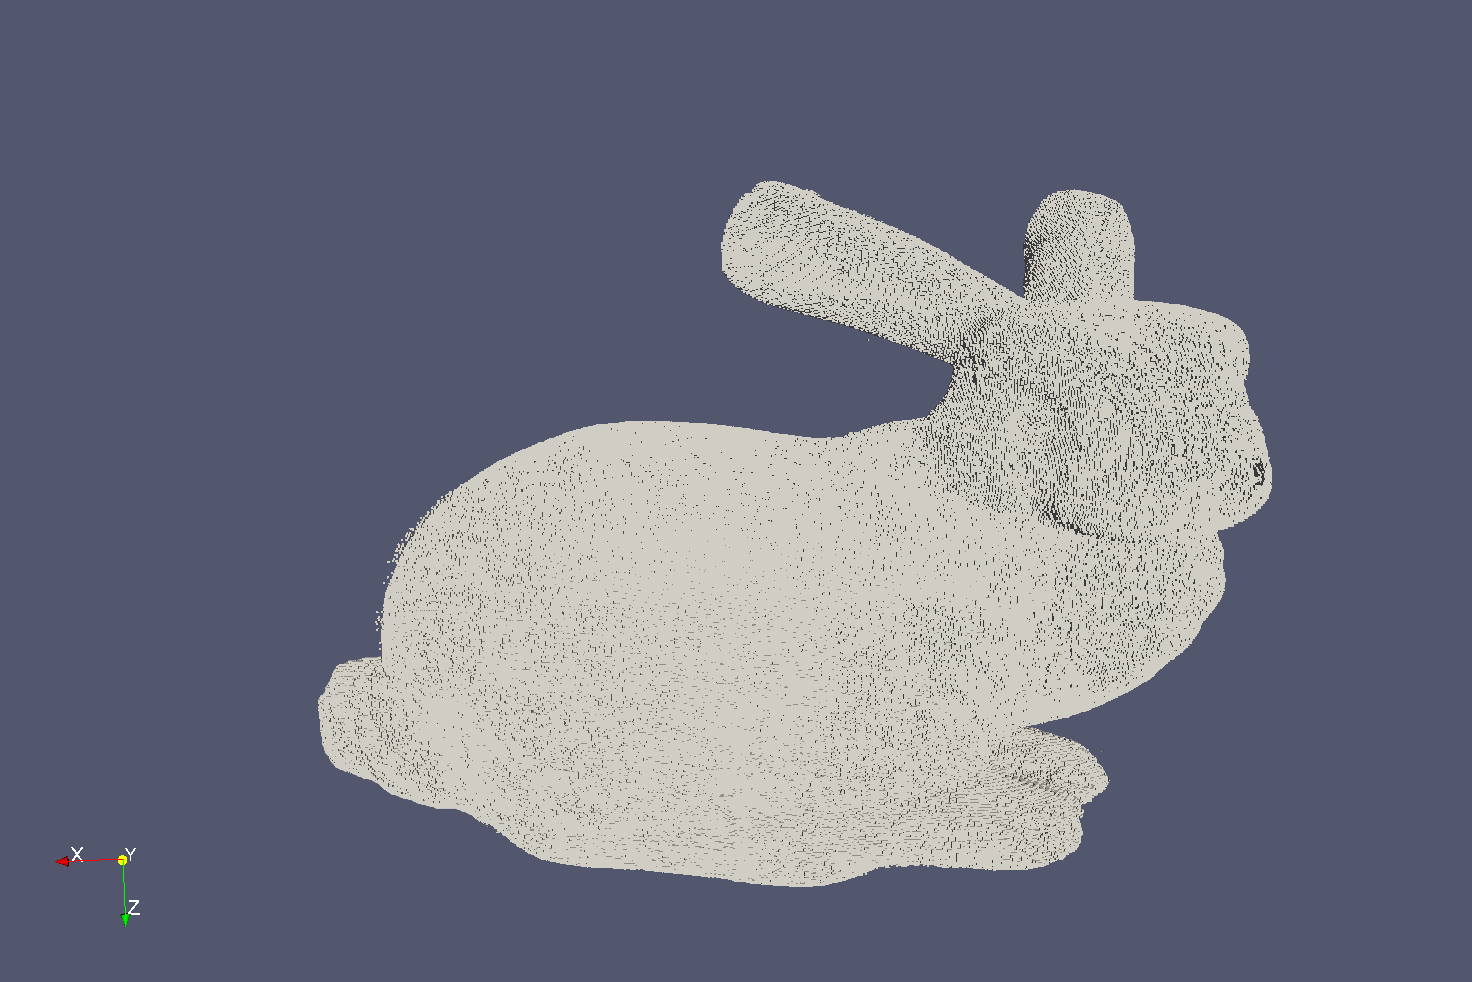
\includegraphics[width=0.49\linewidth]{images/nosmooth3.png}\hfill
   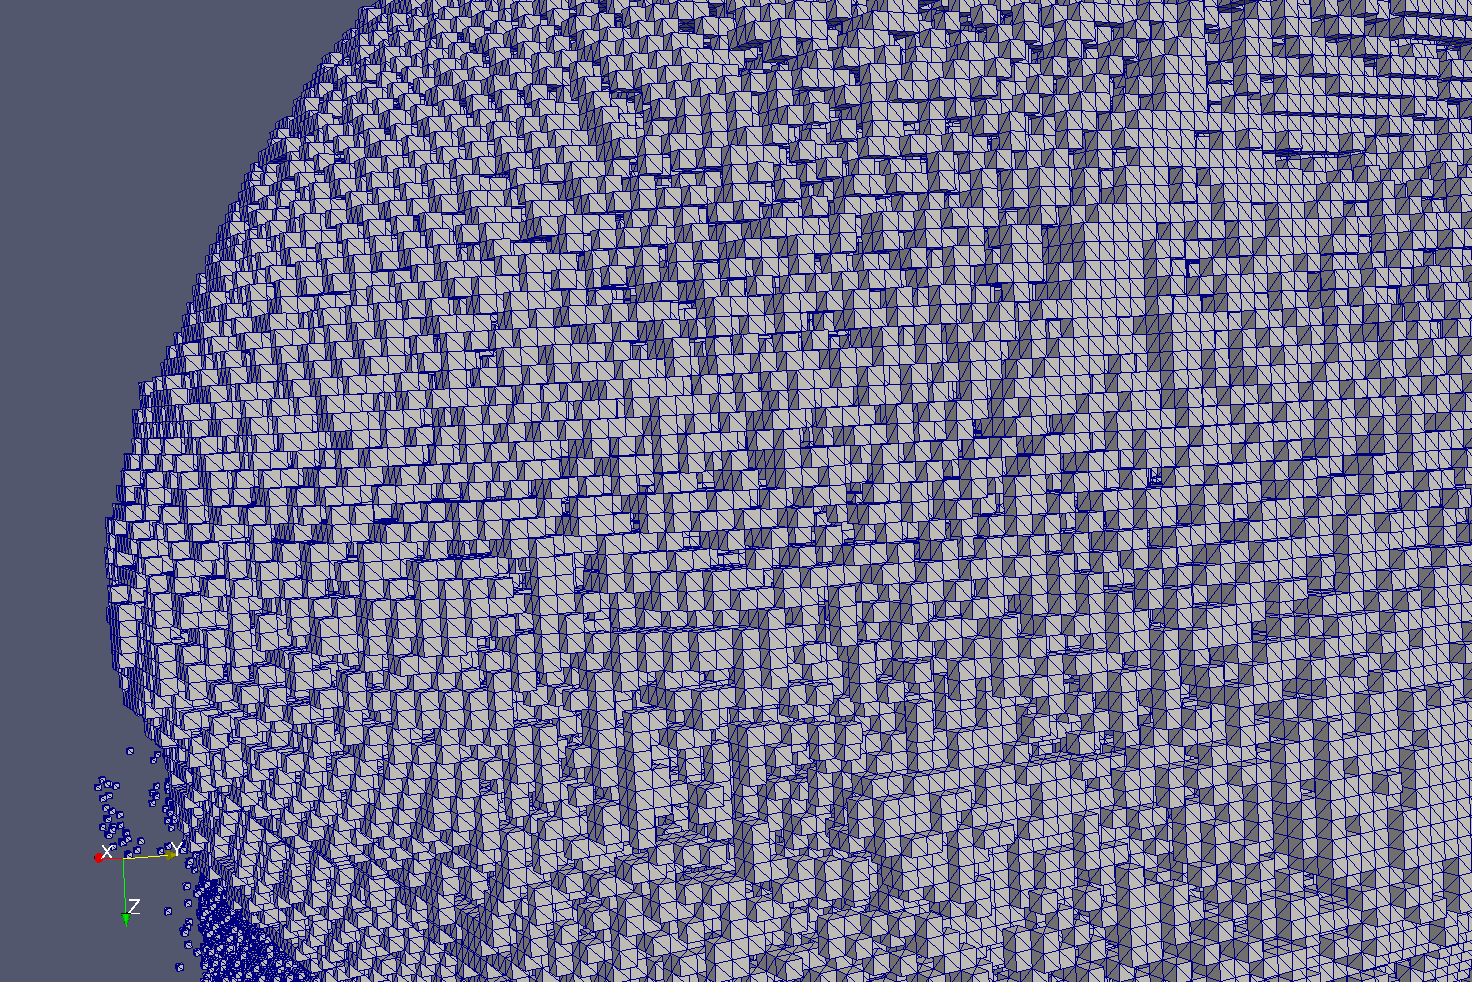
\includegraphics[width=0.49\linewidth]{images/nosmooth4.png}
   \caption[Squared bunny]{Squared bunny}
   \label{fig:squaredBunny}
\end{figure}

The next step of the conversion pipeline solve this problem applying the laplacian smoothing to our bunny. In Figure~\ref{fig:smoothedBunny} we can see the smoothed model.

\begin{figure}[htb] %  figure placement: here, top, bottom
   \centering
   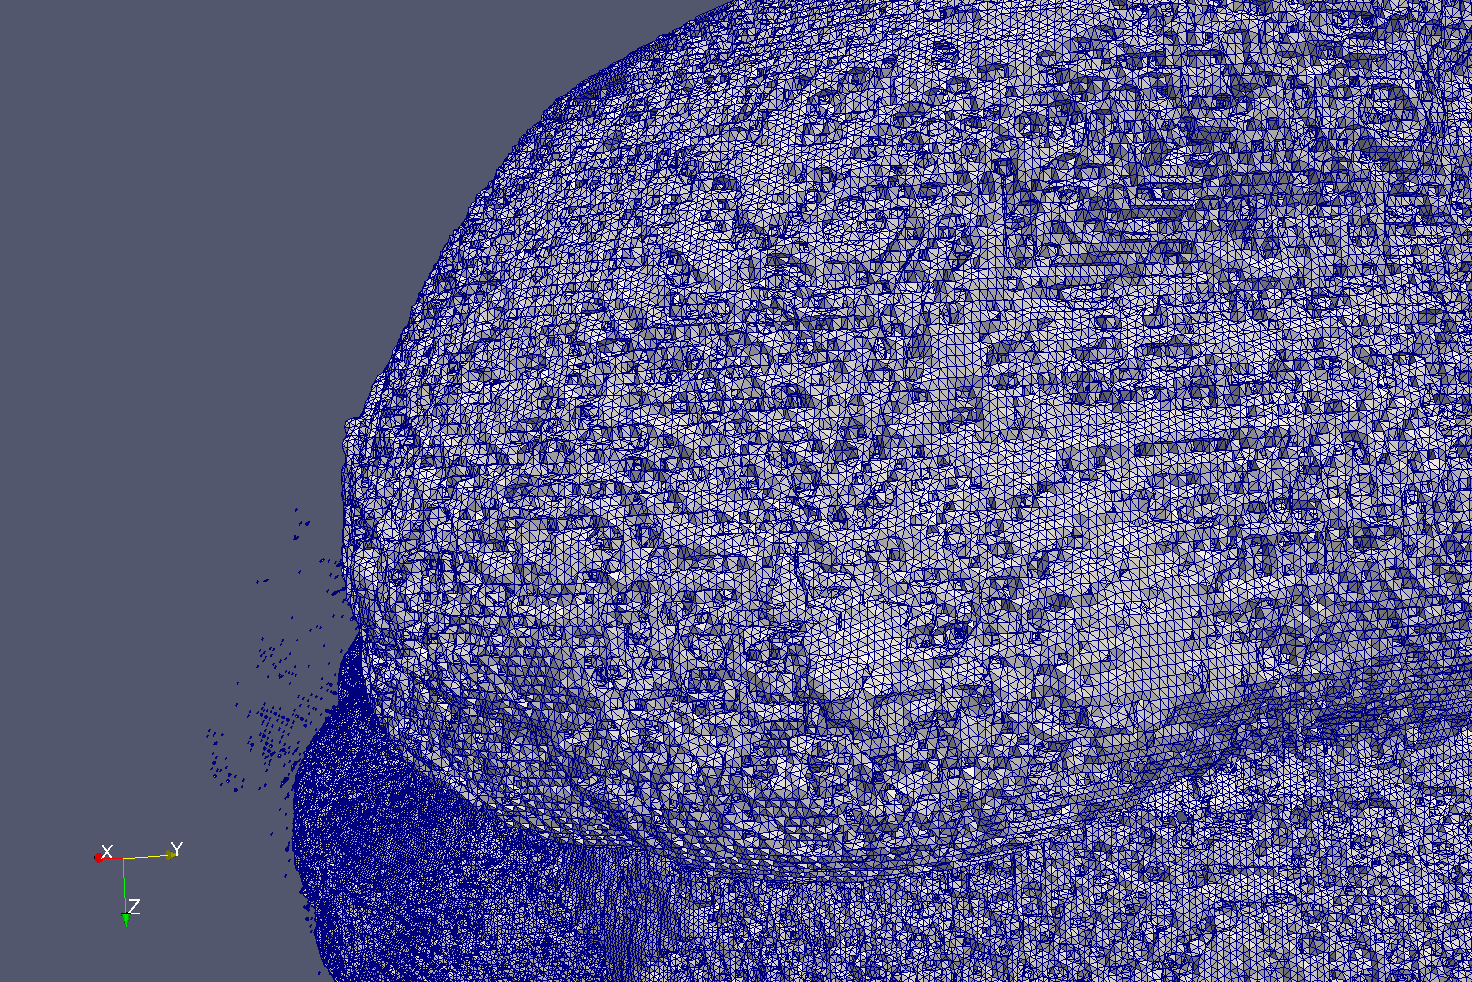
\includegraphics[width=0.49\linewidth]{images/smoothed0.png}\hfill
   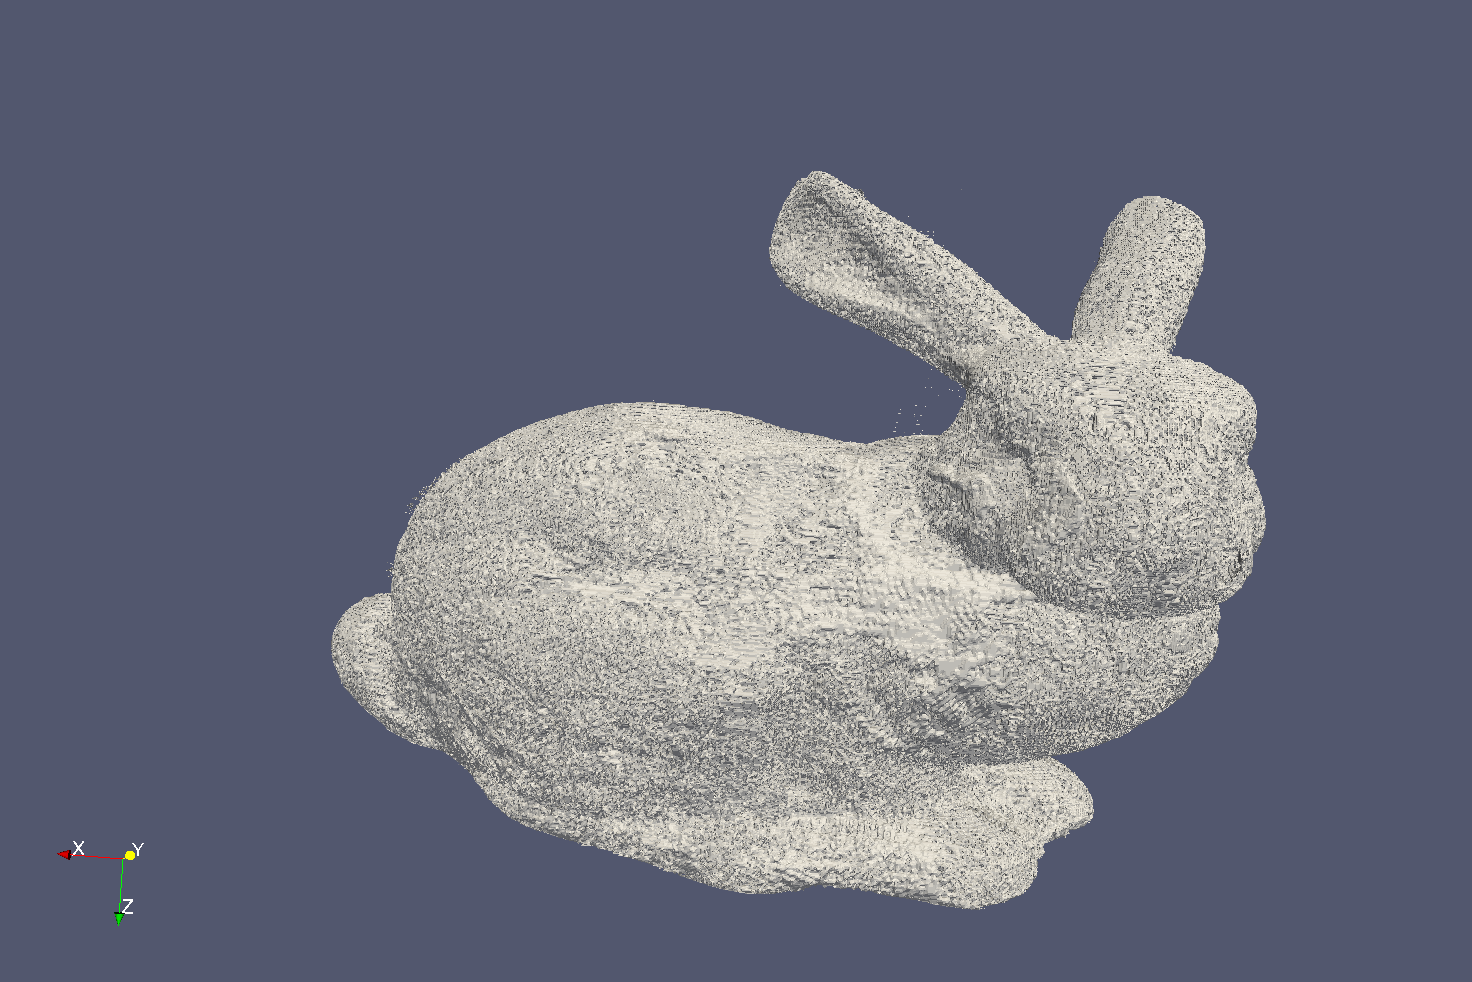
\includegraphics[width=0.49\linewidth]{images/smoothed1.png}\newline
   
   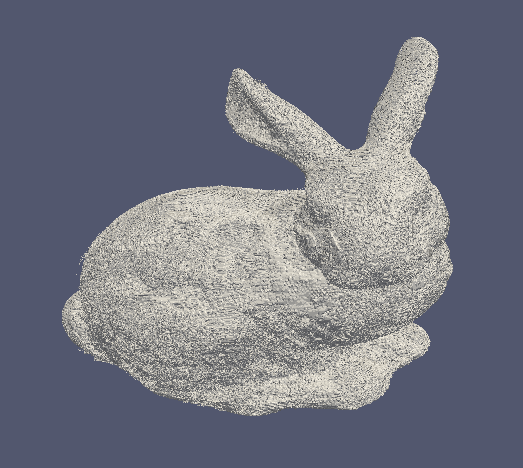
\includegraphics[width=0.49\linewidth]{images/smoothed2.png}\hfill
   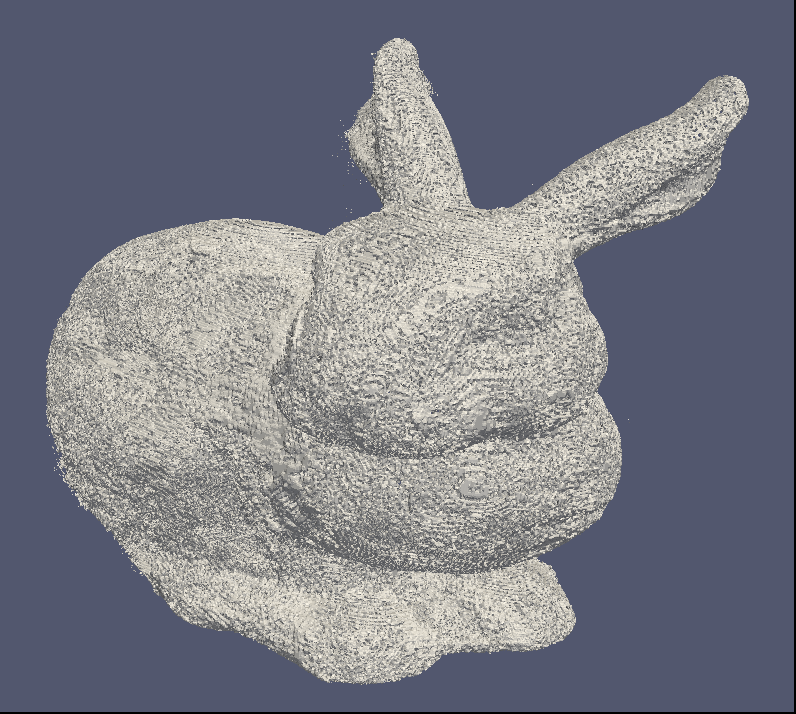
\includegraphics[width=0.49\linewidth]{images/smoothed3.png}
   \caption[Smoothed bunny]{Smoothed bunny}
   \label{fig:smoothedBunny}
\end{figure}

\begin{figure}[htb] %  figure placement: here, top, bottom
   \centering
   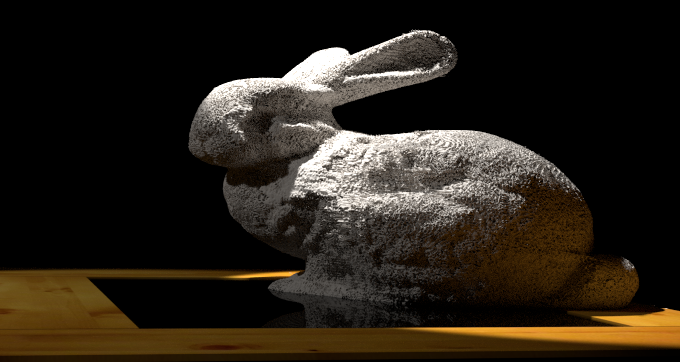
\includegraphics[width=0.90\linewidth]{images/bunnyRendered.png}\hfill
   \caption[Rendering of Stanford bunny]{Rendering of Stanford bunny. This is the same model created above and rendered with Blender}
   \label{fig:renderedBunny}
\end{figure}